\chapter{DATASET DESCRIPTION AND EXPLORATORY DATA ANALYSIS}

\section{Dataset Source}

The data are the Dry Bean dataset (UCI identifier 602), donated to the UCI
Machine Learning Repository on 13 September 2020 and distributed under the
Creative Commons Attribution 4.0 International licence \cite{uci602}. The
archive was downloaded from the official repository URL on 26 November 2026. The
downloaded zip (4,738,776 bytes) has SHA-256 digest
\texttt{0a64eff5be87f48c3dbbfc0a}\allowbreak\texttt{a56c5d5b5167ef8e61cd45d6}\allowbreak
\texttt{9b3e7c7130c06f}, and contains three renderings of the same table: an ARFF
file, an Excel workbook and a plain-text description. The Excel workbook
\texttt{Dry\_Bean\_Dataset.xlsx} (2.9~MB) is the version loaded by the pipeline.
The dataset accompanies the study by Köklü and Özkan \cite{koklu2020}, which
documents the imaging and segmentation procedure that produced the features.
Table~\ref{tab:dataset_summary} records the properties verified from the
downloaded file rather than taken from the repository description.

\begin{table}[htbp]
\centering
\small
\caption{Summary of the dry bean dataset as distributed by UCI}
\label{tab:dataset_summary}
\begin{tabular}{p{0.30\textwidth}p{0.60\textwidth}}
\toprule
Property & Details \\
\midrule
Dataset name & Dry Bean Dataset (UCI ID 602) \\
Provider & UCI Machine Learning Repository \\
Source URL & \url{https://archive.ics.uci.edu/dataset/602/dry+bean+dataset} \\
DOI & 10.24432/C50S4B \\
Date accessed & 2026-11-26 \\
Licence & CC BY 4.0 \\
File format & Excel workbook (.xlsx), also ARFF and TXT \\
Records & 13,611 \\
Columns & 17 (16 features + 1 target) \\
Target variable & Class (7 nominal varieties) \\
Task type & Supervised multiclass classification \\
Missing values & 0 \\
Duplicate rows & 68 \\
Class imbalance ratio & 6.79:1 (majority:minority) \\
\bottomrule
\end{tabular}
\end{table}


Column names are preserved exactly as distributed, including the misspelling
\texttt{AspectRation} in the fifth column. Renaming it would break compatibility
with the published literature and with the file itself, so the original spelling
is used throughout the code and the report.

\section{Dataset Overview}

The workbook contains \DatasetRows{} rows and 17 columns: 16 numeric inputs and
one nominal target. All 16 inputs are numeric with no missing entries; 14 are
stored as floating point and two, \texttt{Area} and \texttt{ConvexArea}, as
integers because they count pixels. The target takes exactly the seven expected
labels, so no relabelling or cleaning of the class column was necessary.

The class counts in Table~\ref{tab:class_counts} show the imbalance that shapes
every later decision. Dermason contributes 26.05\% of the data and Sira 19.37\%,
while Bombay contributes 3.84\%. The majority-to-minority ratio is
\ImbalanceRatio. An accuracy of 90\% is therefore unremarkable on this dataset: a
model that never predicts Bombay loses at most 3.84 percentage points of accuracy
while producing a macro F1 of at most $6/7 \approx 0.857$ on the other classes.

\begin{table}[htbp]
\centering
\small
\caption{Class distribution of the target variable}
\label{tab:class_counts}
\begin{tabular}{clrr}
\toprule
Sl. No. & Variety & Beans & Share (\%) \\
\midrule
1 & Seker & 2,027 & 14.89 \\
2 & Barbunya & 1,322 & 9.71 \\
3 & Bombay & 522 & 3.84 \\
4 & Cali & 1,630 & 11.98 \\
5 & Dermason & 3,546 & 26.05 \\
6 & Horoz & 1,928 & 14.17 \\
7 & Sira & 2,636 & 19.37 \\
\midrule
 & Total & 13,611 & 100.00 \\
\bottomrule
\end{tabular}
\end{table}


\section{Attribute Description}

The 16 descriptors are geometric measurements of the segmented bean mask, and
they are not independent by construction: several are algebraic functions of the
same primitive quantities. Table~\ref{tab:attributes} lists them with their
definitions. Writing $A$ for area, $P$ for perimeter, $L$ and $l$ for the major
and minor axis lengths, $C$ for convex area and $E_d$ for the equivalent
diameter, the four shape factors distributed with the dataset are
\begin{align}
  \text{roundness} &= \frac{4\pi A}{P^{2}}, &
  \text{Compactness} &= \frac{E_d}{L}, \label{eq:roundness}\\
  \text{ShapeFactor1} &= \frac{A}{L^{3}}, &
  \text{ShapeFactor2} &= \frac{l}{L}, \\
  \text{ShapeFactor3} &= \frac{A}{L\,l}, &
  \text{ShapeFactor4} &= \frac{A}{C}\ \text{(hull roundness)}.
\end{align}
Because $E_d = 2\sqrt{A/\pi}$, the compactness can be rewritten as
$2\sqrt{A/\pi}/L$, which makes the redundancy between the size features and the
shape factors explicit. This algebraic coupling, not measurement error, is the
origin of the high correlations reported in Section~3.4.6.

\begin{table}[htbp]
\centering
\footnotesize
\caption{Attributes of the dataset, in the order distributed by UCI}
\label{tab:attributes}
\begin{tabular}{clp{0.17\textwidth}p{0.36\textwidth}c}
\toprule
No. & Attribute & Type & Description & Role \\
\midrule
1 & Area & Integer & Pixels inside the bean boundary & Input \\
2 & Perimeter & Continuous & Length of the bean boundary & Input \\
3 & MajorAxisLength & Continuous & Longest line through the bean & Input \\
4 & MinorAxisLength & Continuous & Shortest line through the bean & Input \\
5 & AspectRation & Continuous & MajorAxisLength / MinorAxisLength & Input \\
6 & Eccentricity & Continuous & Eccentricity of the equivalent ellipse & Input \\
7 & ConvexArea & Integer & Pixels in the smallest enclosing convex polygon & Input \\
8 & EquivDiameter & Continuous & Diameter of a circle of equal area & Input \\
9 & Extent & Continuous & Bean area / bounding-box area & Input \\
10 & Solidity & Continuous & Bean area / convex hull area & Input \\
11 & roundness & Continuous & 4 pi Area / Perimeter squared & Input \\
12 & Compactness & Continuous & EquivDiameter / MajorAxisLength & Input \\
13 & ShapeFactor1 & Continuous & Area / MajorAxisLength cubed & Input \\
14 & ShapeFactor2 & Continuous & MinorAxisLength / MajorAxisLength & Input \\
15 & ShapeFactor3 & Continuous & Area / (Major x Minor axis length) & Input \\
16 & ShapeFactor4 & Continuous & Convex-hull based roundness ratio & Input \\
17 & Class & Nominal & One of seven registered bean varieties & Target \\
\bottomrule
\end{tabular}
\end{table}


\section{Exploratory Data Analysis}

\subsection{Class distribution}

Figure~\ref{fig:class_distribution} shows the counts with their shares. The
distribution is unimodal and moderately skewed, with no class below 500 beans.
That lower bound is what makes stratified splitting and macro-averaged metrics
sufficient: there is enough data to estimate a per-class F1 for Bombay, but not
enough to tolerate a split that under-represents it.

\begin{figure}[htbp]
\centering
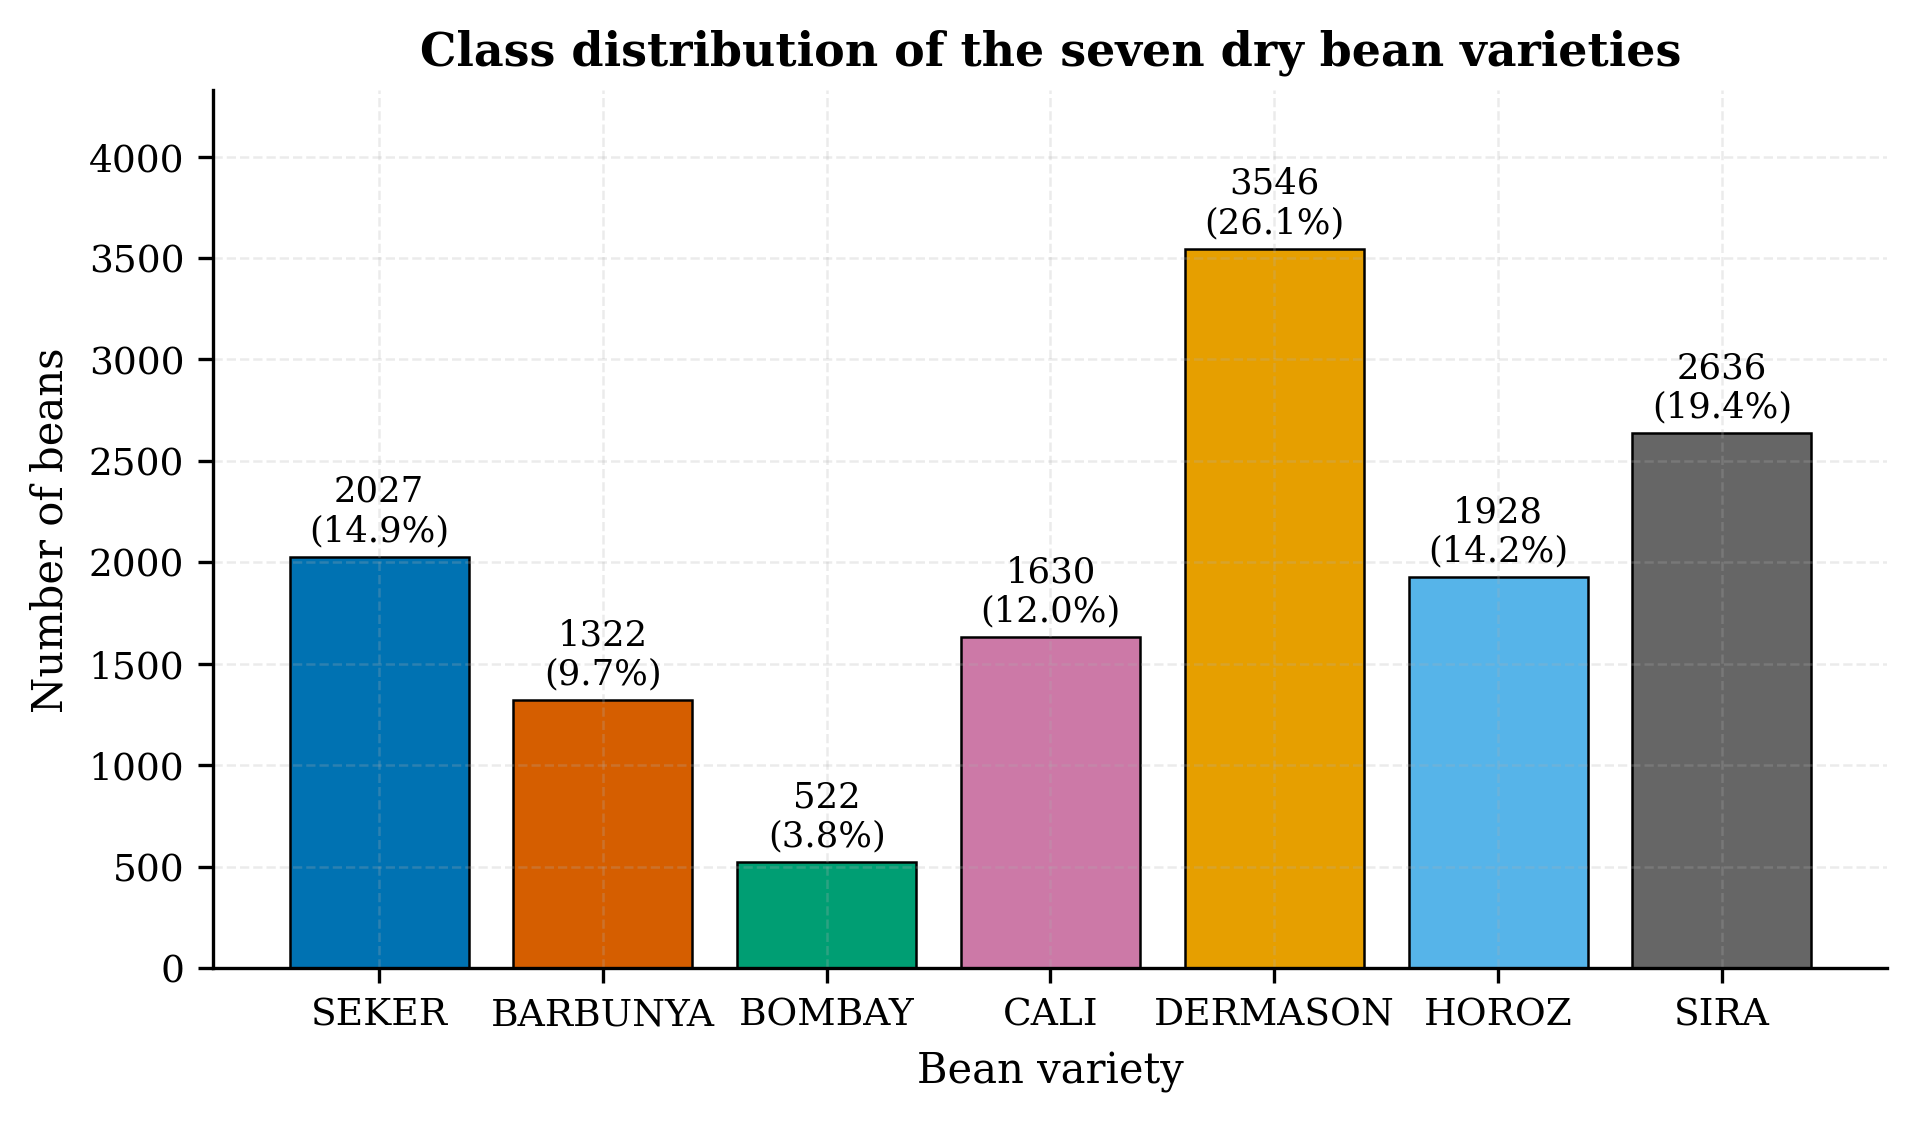
\includegraphics[width=0.70\textwidth]{fig_3_1_class_distribution.png}
\caption{Class distribution of the seven dry bean varieties. Counts and shares are
annotated; the smallest class, Bombay, supplies 3.84\% of the data.}
\label{fig:class_distribution}
\end{figure}

\subsection{Data completeness}

Every one of the 16 features is 100\% populated, as shown in
Figure~\ref{fig:missing}. There are also no infinite values, no negative values
and no constant columns. The completeness matters for the modelling stage: no
imputation is required, and the preprocessing pipeline therefore contains only a
scaler, which removes an entire class of leakage risks. A separate observation is
that \DuplicateRows{} rows are exact repeats of an earlier row across all 17
columns. They are discussed in Section~4.1 and were retained.

\begin{figure}[htbp]
\centering
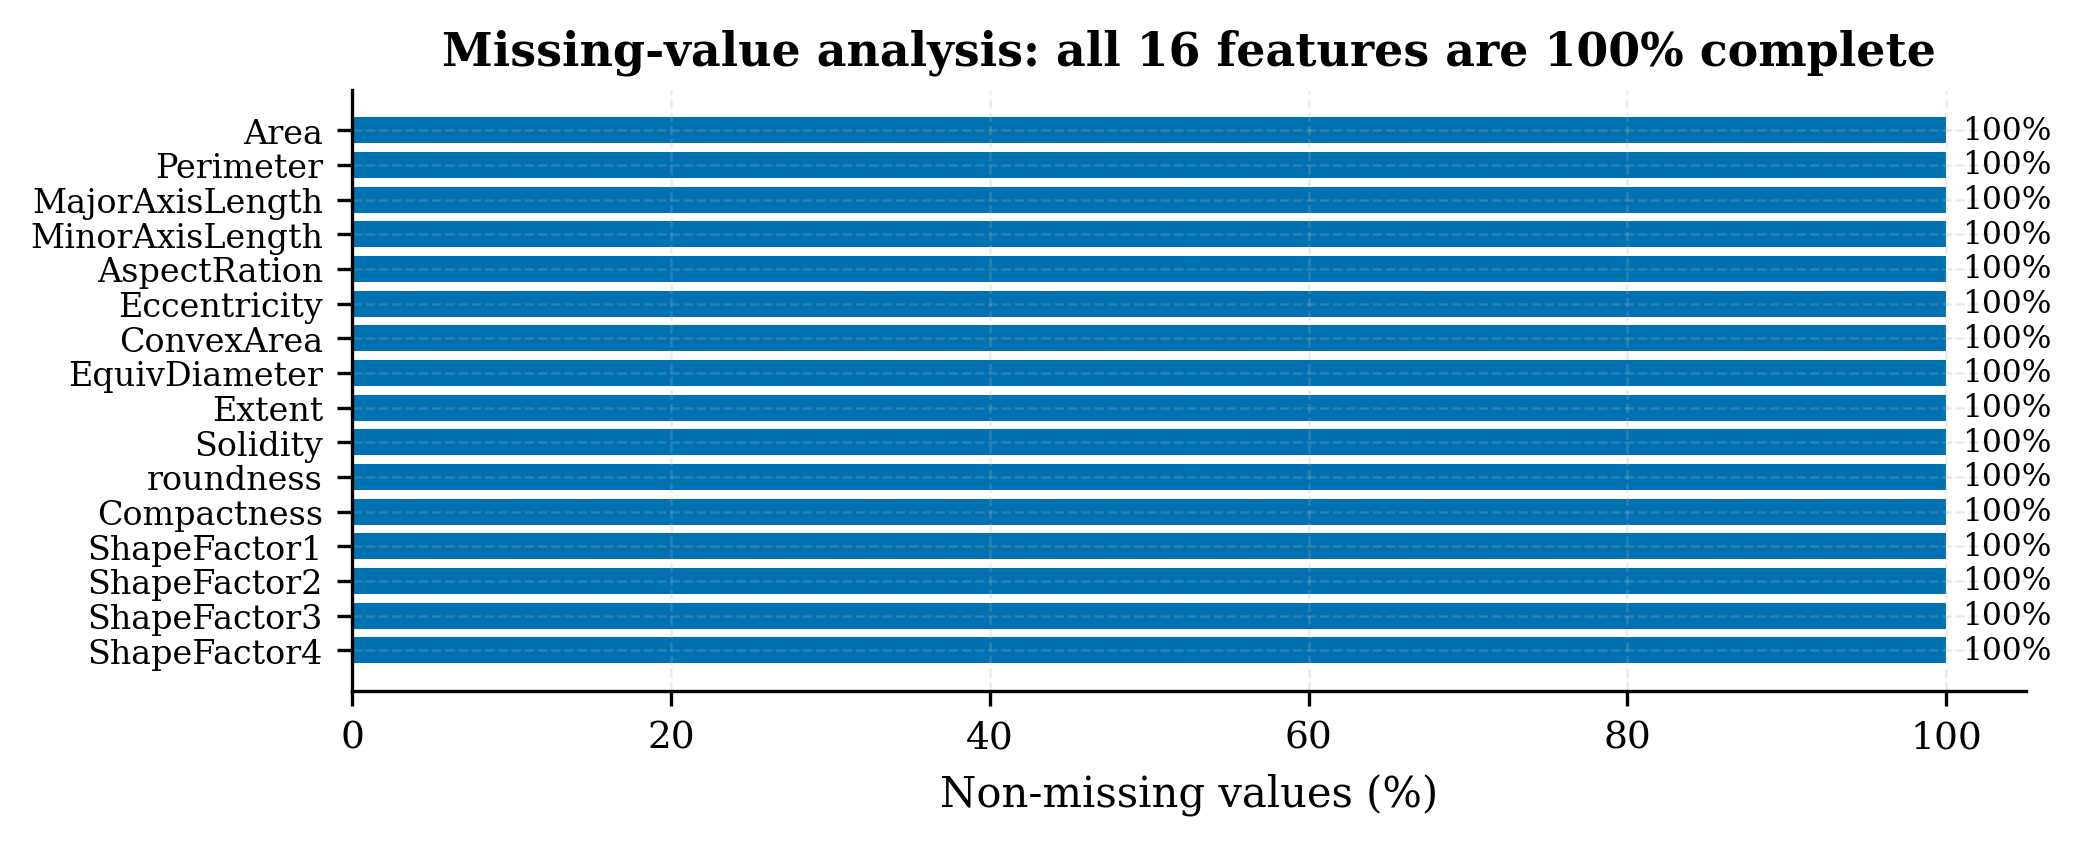
\includegraphics[width=0.60\textwidth]{fig_3_2_missing_values.png}
\caption{Missing-value analysis. All 16 features are complete, so no imputation
step is needed anywhere in the pipeline.}
\label{fig:missing}
\end{figure}

\subsection{Descriptive statistics}

Table~\ref{tab:descriptive} summarises the 16 features. Three properties govern
the preprocessing choices. The scales differ by four orders of magnitude:
\texttt{Area} has a mean of 53,048 pixels, while \texttt{ShapeFactor2} has a mean
of 0.002. Several features are strongly right-skewed (\texttt{Area} 2.95,
\texttt{ConvexArea} 2.94, \texttt{Solidity} $-$2.55, \texttt{ShapeFactor4}
$-$2.76), and the two bounded descriptors, \texttt{Solidity} and
\texttt{ShapeFactor4}, pile up against their upper limit. \texttt{Solidity} has a
standard deviation of 0.005, so almost all of its variance lies between 0.97 and
1.00.

\begin{table}[htbp]
\centering
\footnotesize
\caption{Descriptive statistics of the 16 morphological features (n = 13,611)}
\label{tab:descriptive}
\begin{tabular}{lrrrrrr}
\toprule
Feature & Mean & Std. dev. & Min & Median & Max & Skew \\
\midrule
Area & 5.305e+04 & 2.932e+04 & 2.042e+04 & 4.465e+04 & 2.546e+05 & 2.95 \\
Perimeter & 855.3 & 214.3 & 524.7 & 794.9 & 1985 & 1.63 \\
MajorAxisLength & 320.1 & 85.69 & 183.6 & 296.9 & 738.9 & 1.36 \\
MinorAxisLength & 202.3 & 44.97 & 122.5 & 192.4 & 460.2 & 2.24 \\
AspectRation & 1.583 & 0.2467 & 1.025 & 1.551 & 2.43 & 0.58 \\
Eccentricity & 0.7509 & 0.092 & 0.219 & 0.7644 & 0.9114 & -1.06 \\
ConvexArea & 5.377e+04 & 2.977e+04 & 2.068e+04 & 4.518e+04 & 2.633e+05 & 2.94 \\
EquivDiameter & 253.1 & 59.18 & 161.2 & 238.4 & 569.4 & 1.95 \\
Extent & 0.7497 & 0.0491 & 0.5553 & 0.7599 & 0.8662 & -0.90 \\
Solidity & 0.9871 & 0.0047 & 0.9192 & 0.9883 & 0.9947 & -2.55 \\
roundness & 0.8733 & 0.0595 & 0.4896 & 0.8832 & 0.9907 & -0.64 \\
Compactness & 0.7999 & 0.0617 & 0.6406 & 0.8013 & 0.9873 & 0.04 \\
ShapeFactor1 & 0.0066 & 0.0011 & 0.0028 & 0.0066 & 0.0105 & -0.53 \\
ShapeFactor2 & 0.0017 & 0.0006 & 0.0006 & 0.0017 & 0.0037 & 0.30 \\
ShapeFactor3 & 0.6436 & 0.099 & 0.4103 & 0.642 & 0.9748 & 0.24 \\
ShapeFactor4 & 0.9951 & 0.0044 & 0.9477 & 0.9964 & 0.9997 & -2.76 \\
\bottomrule
\end{tabular}
\end{table}


The practical consequence is that magnitude-based algorithms cannot consume these
columns raw: a Euclidean distance computed on unscaled values is, to within
rounding, a distance in \texttt{Area} alone. Section~4.2 addresses this with a
standard scaler inside a pipeline.

\subsection{Univariate distributions}

Figure~\ref{fig:histograms} shows all 16 histograms with their skewness. Three
groups are visible. The size features (\texttt{Area}, \texttt{Perimeter},
\texttt{ConvexArea}, \texttt{EquivDiameter} and the two axis lengths) are
right-skewed with a long upper tail, which is the signature of a mixture: the bulk
of the beans plus a small, distinctly larger group. The shape factors are
smoother and often bimodal. The bounded ratios (\texttt{Extent},
\texttt{Solidity}, \texttt{ShapeFactor4}) are concentrated near their ceilings.

The bimodality is not noise. It is the first indication that at least one variety
occupies a separate region of the size space, which the class-wise plots confirm.

\begin{figure}[htbp]
\centering
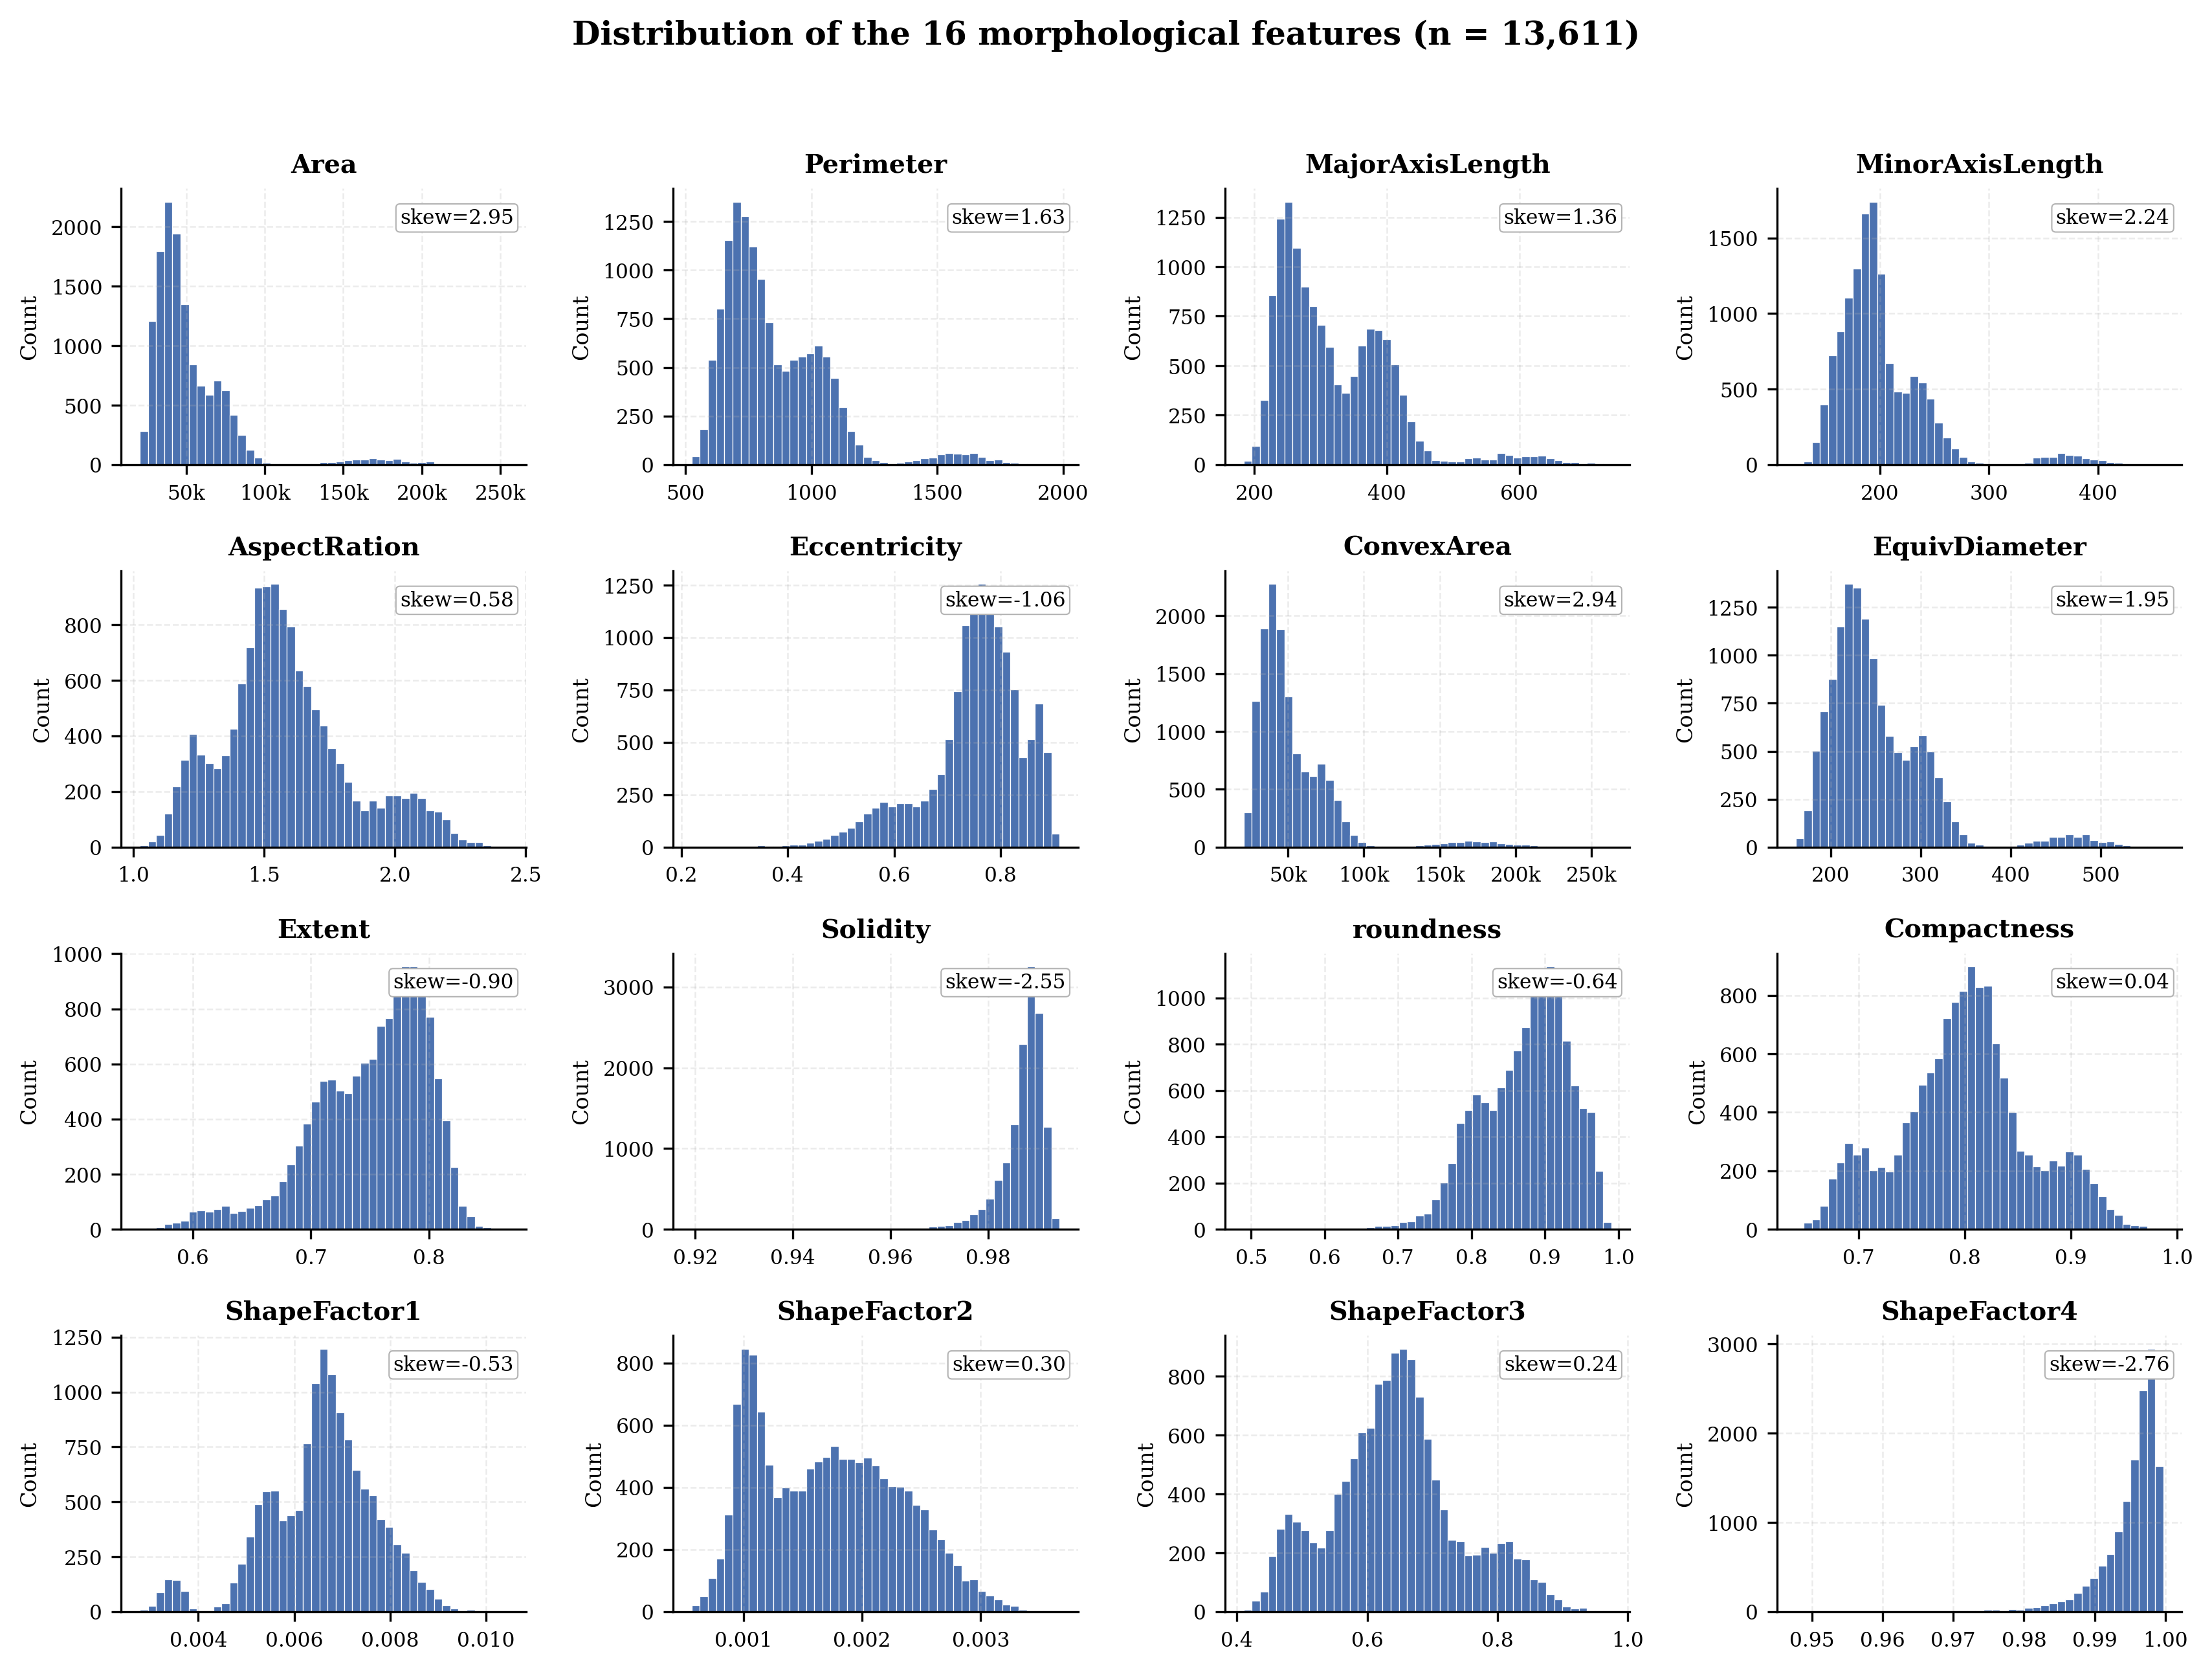
\includegraphics[width=0.95\textwidth]{fig_3_3_feature_histograms.png}
\caption{Distribution of the 16 morphological features. Skewness is annotated in
each panel. Size features are right-skewed; several shape factors are bimodal.}
\label{fig:histograms}
\end{figure}

\subsection{Class-wise distributions}

Figure~\ref{fig:boxplots} breaks eight features down by variety, and
Figure~\ref{fig:violin} shows the density of four of them. The separation is
uneven. \texttt{Area} isolates Bombay completely: its mean area of 173,485
pixels is 2.4 times that of Barbunya, the next largest, and no other variety
reaches its lower quartile. Dermason is the smallest at 32,119 pixels. The
remaining five varieties form a band between roughly 39,000 and 76,000 pixels
where the ranges overlap almost completely.

Shape separates what size cannot. Seker is the roundest variety
(\texttt{roundness} mean 0.945, \texttt{Compactness} 0.897, eccentricity 0.585),
while Horoz is the most elongated (\texttt{Compactness} 0.701, eccentricity
0.867, \texttt{Extent} 0.706). Cali and Barbunya have similar areas (75,538 and
69,804 pixels) but differ in compactness (0.757 against 0.805), which is exactly
the kind of distinction that a classifier must learn from a ratio rather than
from a magnitude.

\begin{figure}[htbp]
\centering
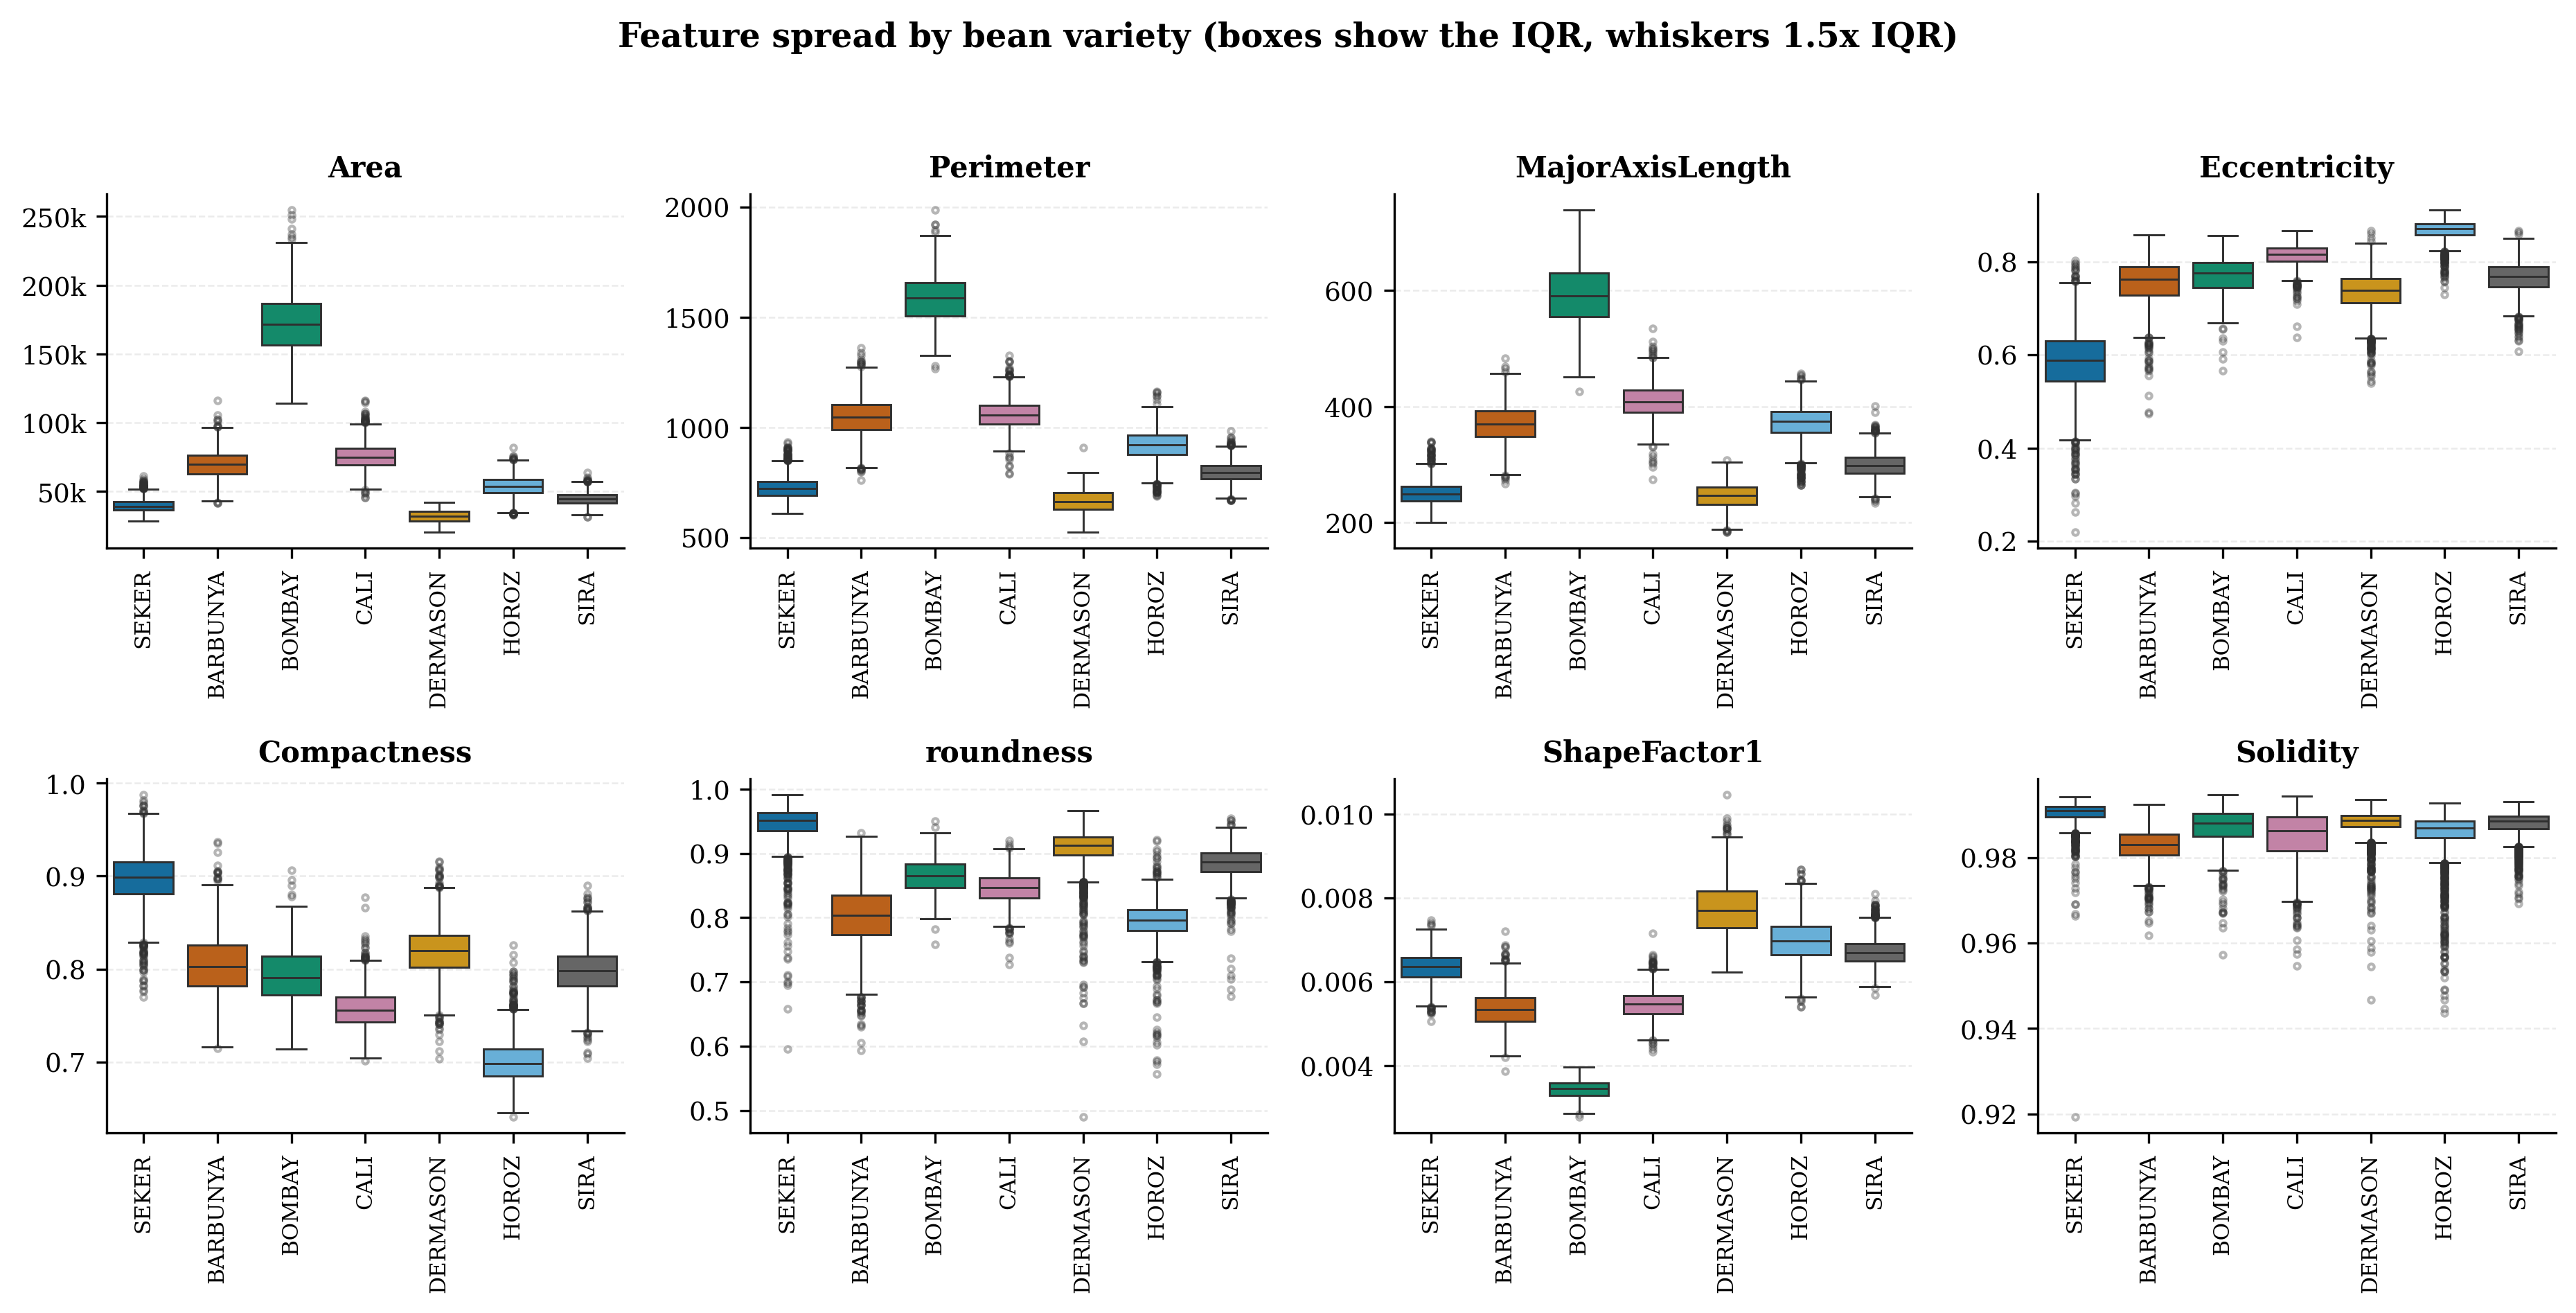
\includegraphics[width=0.95\textwidth]{fig_3_4_boxplots_by_class.png}
\caption{Feature spread by variety. Bombay is separated by every size feature;
the other six overlap and require shape information.}
\label{fig:boxplots}
\end{figure}

\begin{figure}[htbp]
\centering
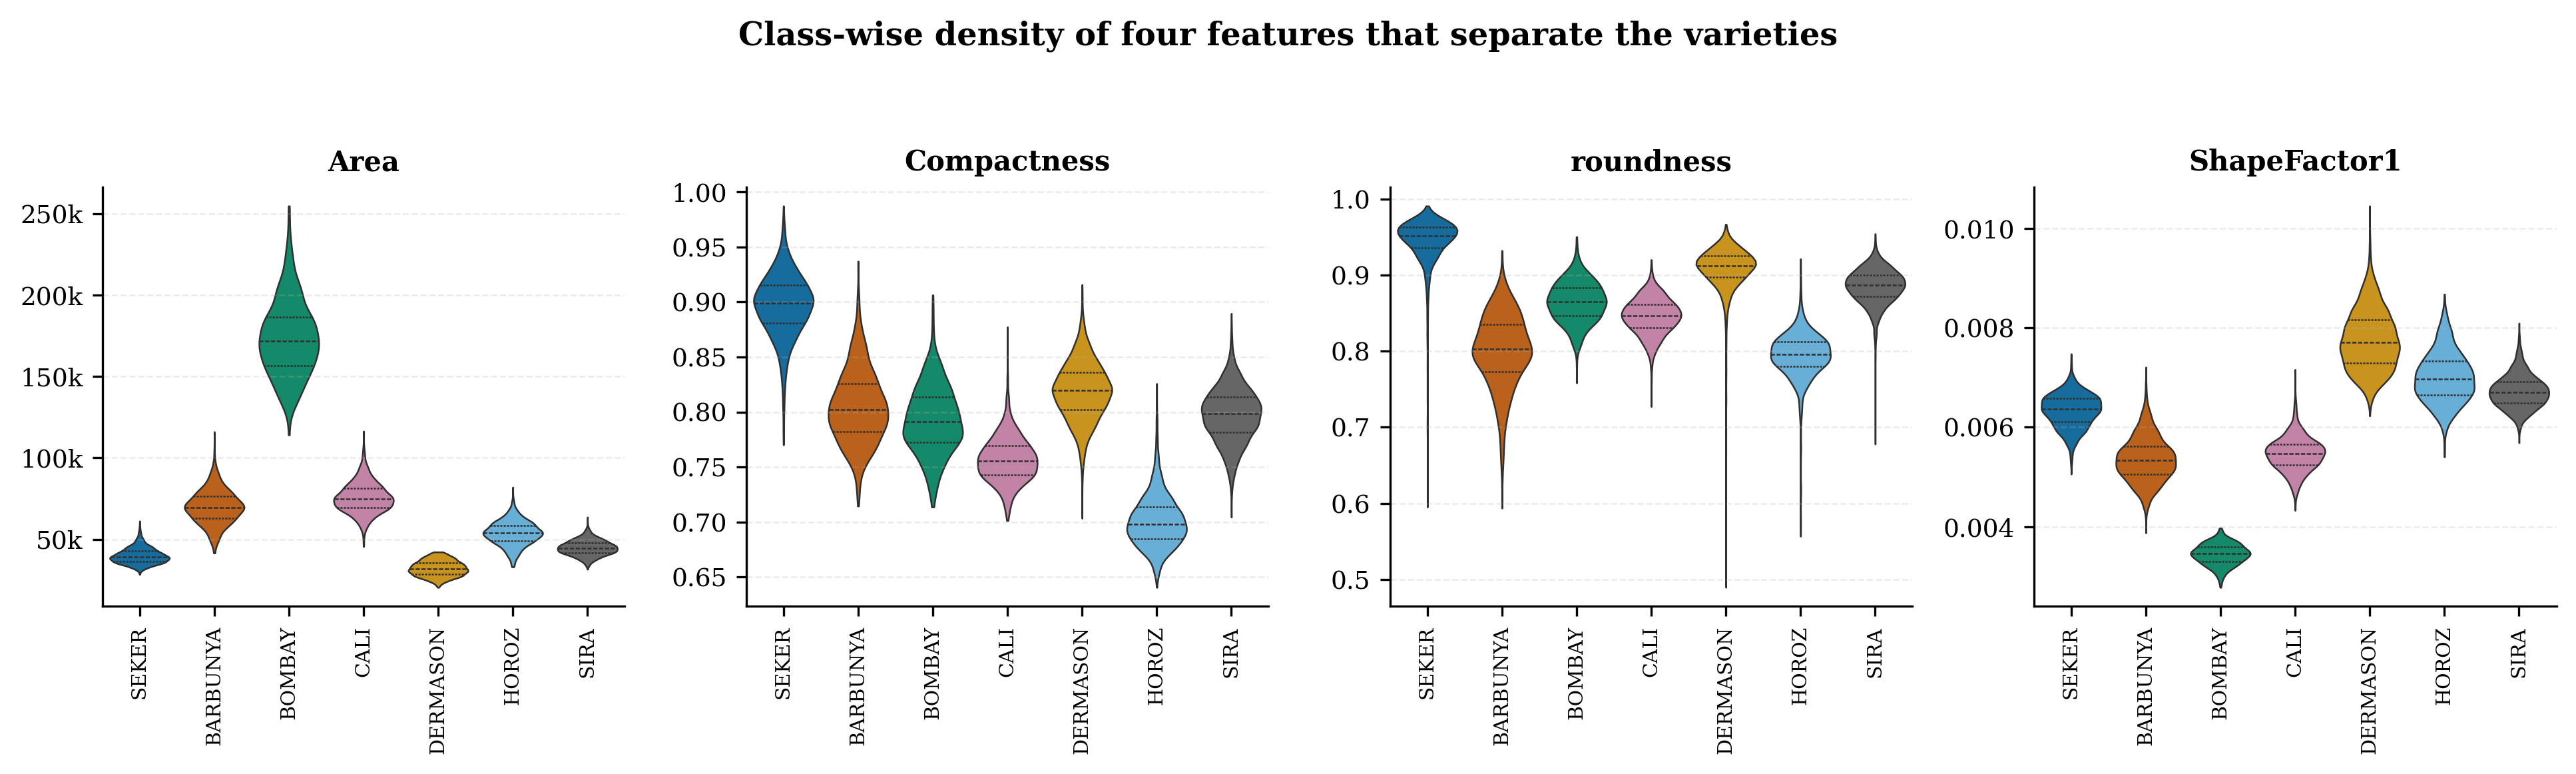
\includegraphics[width=0.90\textwidth]{fig_3_7_classwise_comparison.png}
\caption{Class-wise density of four informative features. Seker concentrates at
high roundness, Horoz at low compactness, and Bombay sits alone at low
ShapeFactor1.}
\label{fig:violin}
\end{figure}

\subsection{Correlation structure}

Figure~\ref{fig:corr} is the Pearson correlation matrix and
Table~\ref{tab:corr_pairs} lists the ten strongest pairs. Twenty-one pairs exceed
$|r| = 0.90$. \texttt{Area} and \texttt{ConvexArea} are effectively the same
variable ($r = 0.9999$), which is expected because a bean is nearly convex and
its convex hull therefore covers almost the same pixels. \texttt{Compactness} and
\texttt{ShapeFactor3} reach $-0.9987$, and \texttt{Perimeter} correlates with
\texttt{EquivDiameter} at 0.9914.

Two decisions follow. First, the multicollinearity is real and will affect the
interpretation of feature importance: when two columns carry the same
information, an impurity-based or permutation-based importance can split the
credit arbitrarily between them. Chapter~6 reports this caveat with the results
rather than ignoring it. Second, the correlation is \emph{not} treated as a reason
to delete columns. A tree ensemble can still exploit the small residual
difference between \texttt{Area} and \texttt{ConvexArea}, and the ablation in
Section~6.4 measures the cost of removing the redundant cluster instead of
assuming it.

\begin{figure}[htbp]
\centering
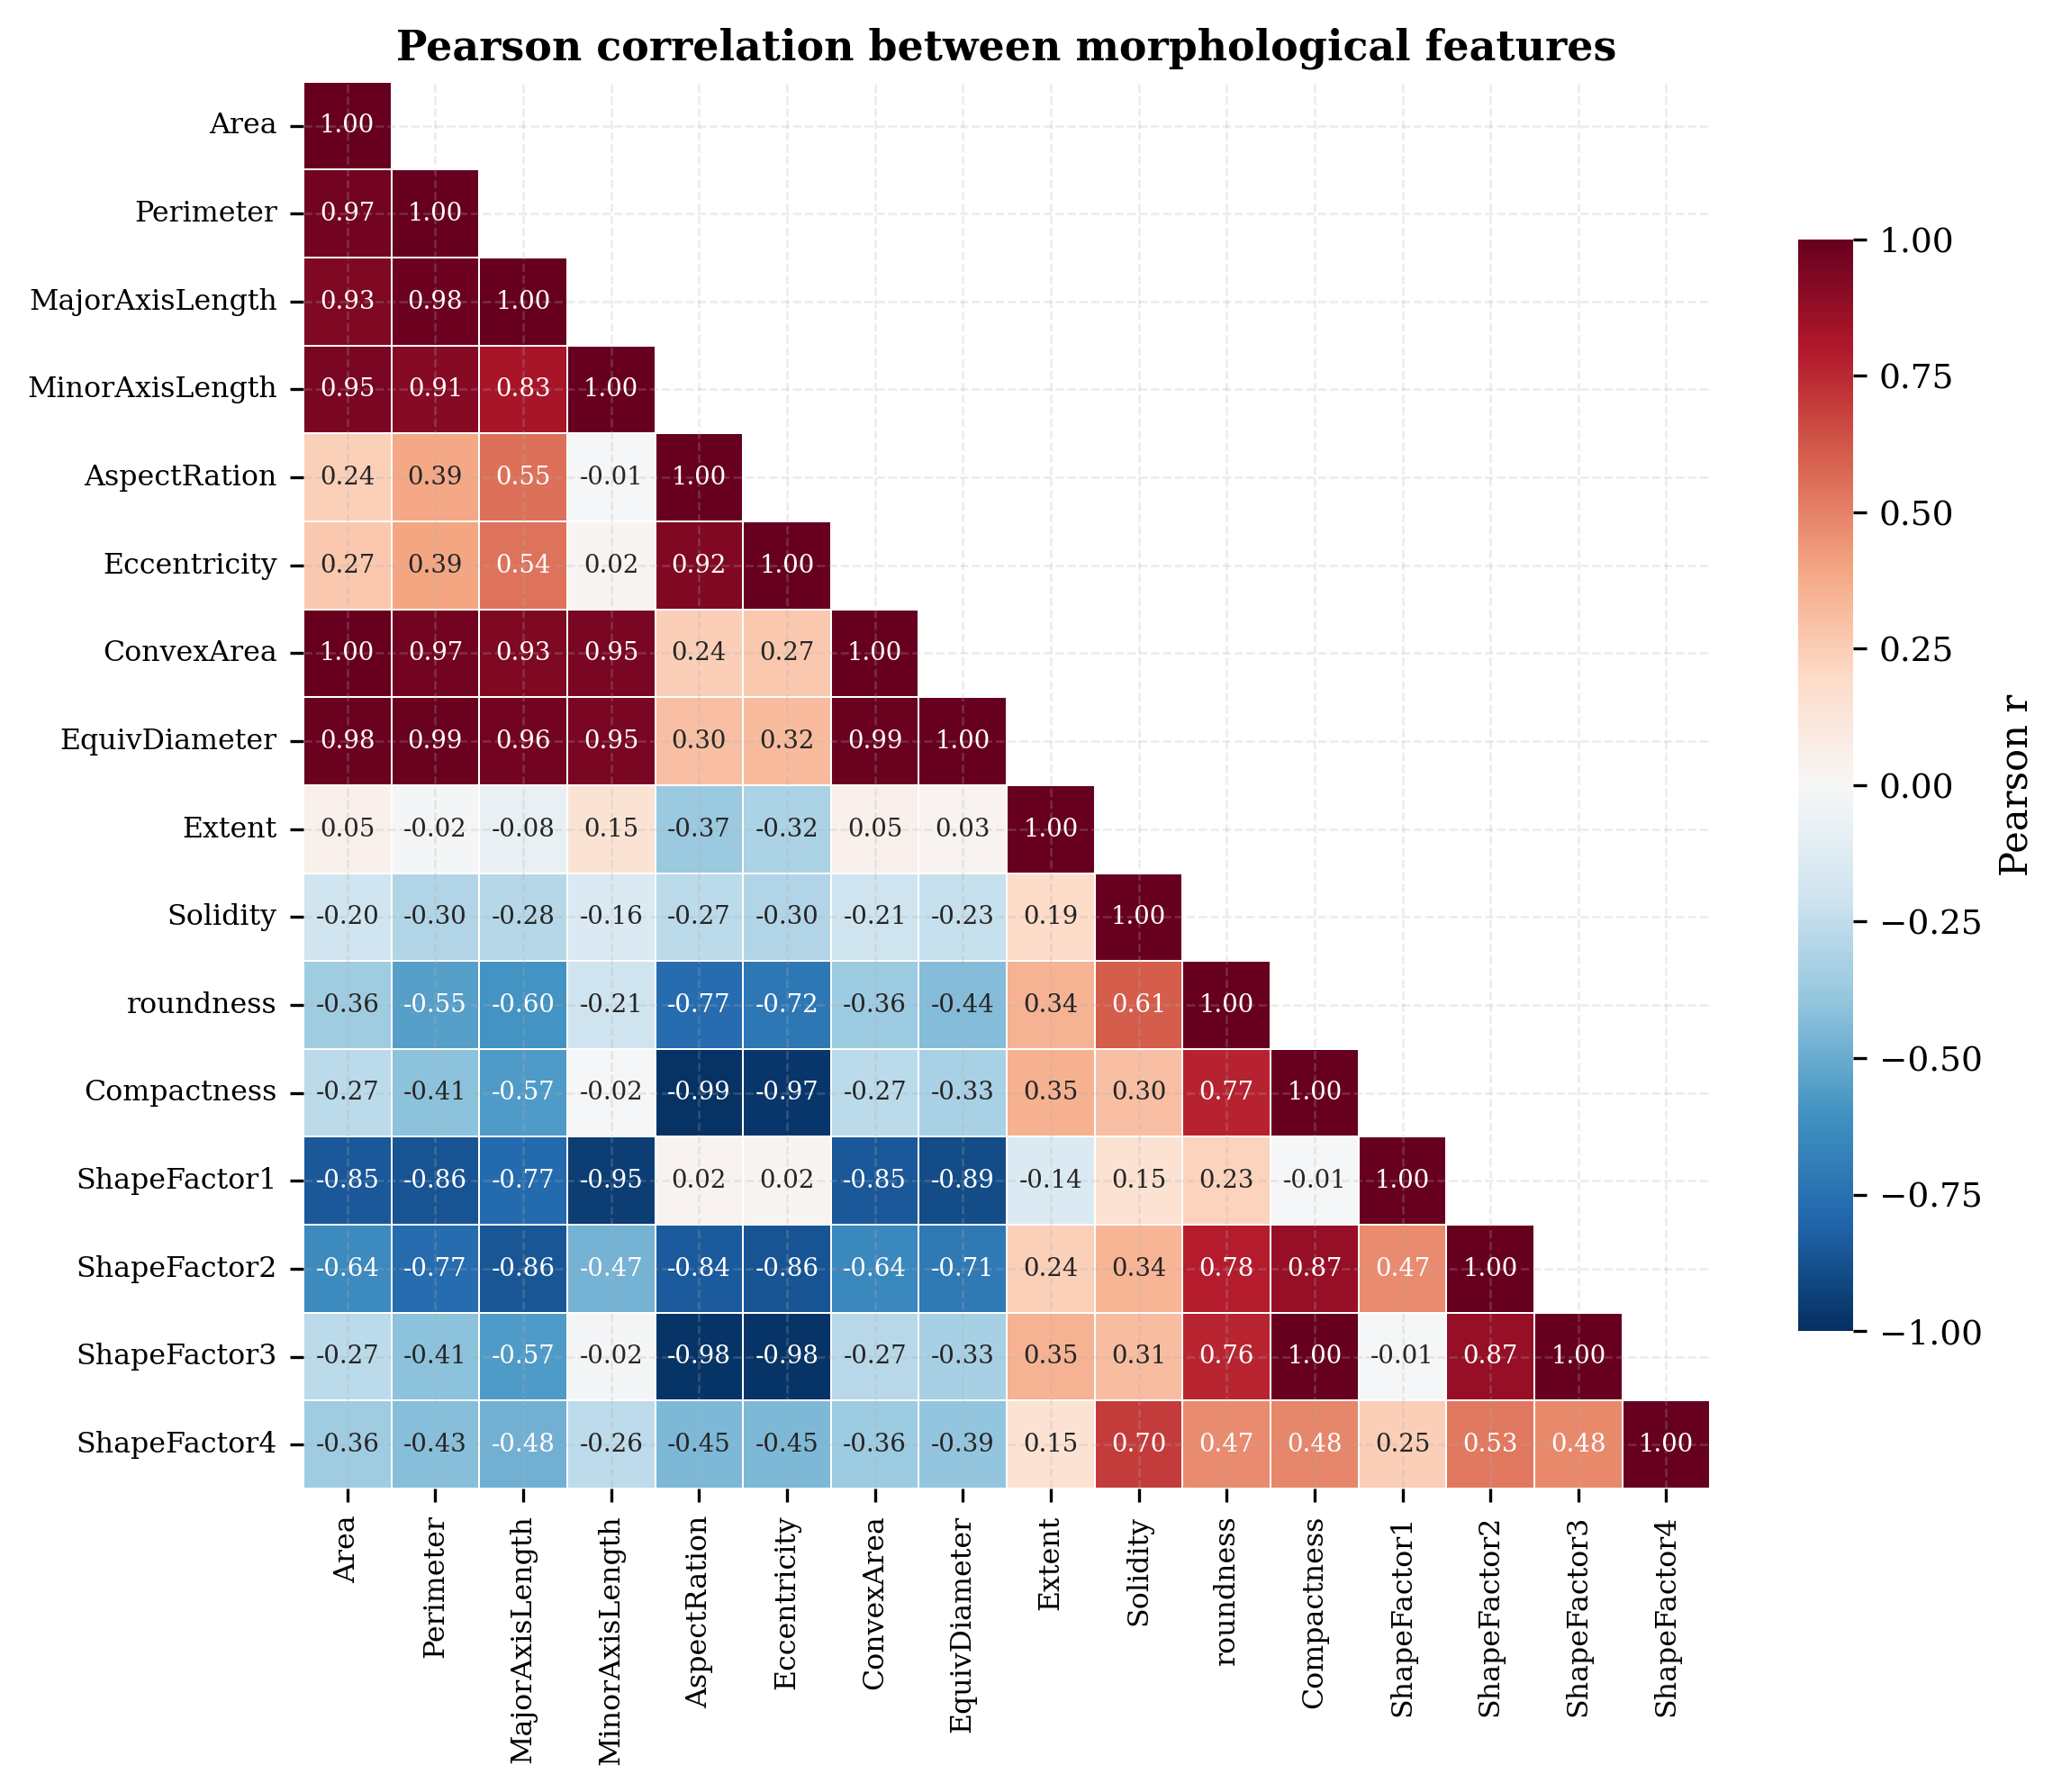
\includegraphics[width=0.62\textwidth]{fig_3_5_correlation_heatmap.png}
\caption{Pearson correlation between the 16 features. The lower triangle is shown;
21 pairs exceed $|r| = 0.90$.}
\label{fig:corr}
\end{figure}

\begin{table}[htbp]
\centering
\small
\caption{The ten strongest feature correlations (all 21 pairs above 0.90 are listed in Appendix B)}
\label{tab:corr_pairs}
\begin{tabular}{lr}
\toprule
Feature pair & Pearson r \\
\midrule
Area -- ConvexArea & +0.9999 \\
Compactness -- ShapeFactor3 & +0.9987 \\
Perimeter -- EquivDiameter & +0.9914 \\
AspectRation -- Compactness & -0.9877 \\
ConvexArea -- EquivDiameter & +0.9852 \\
Area -- EquivDiameter & +0.9850 \\
Eccentricity -- ShapeFactor3 & -0.9811 \\
AspectRation -- ShapeFactor3 & -0.9786 \\
Perimeter -- MajorAxisLength & +0.9773 \\
Eccentricity -- Compactness & -0.9703 \\
\bottomrule
\end{tabular}
\end{table}


\subsection{Multivariate relationships}

The pair plot in Figure~\ref{fig:pairplot} is the clearest single view of the
problem. Bombay forms an isolated cluster at high area and high perimeter.
Dermason forms a second, low-area cluster. The remaining five varieties occupy one
dense cloud whose internal structure is weak: Cali and Barbunya overlap almost
completely, and Sira sits between them and Dermason. Figure~\ref{fig:scatter}
shows the same structure in two dimensions and makes the practical consequence
visible: \texttt{Area} against \texttt{Perimeter} is nearly a straight line,
because both measure size, whereas \texttt{Compactness} against \texttt{roundness}
is the plane in which the five overlapping varieties actually differ.

Two adjacencies are visible inside the cloud and both matter later. Cali
(mean area 75,538, compactness 0.757) and Barbunya (69,804, 0.805) occupy the same
size band and differ mainly in how elongated they are. Dermason (32,119, 0.819)
and Sira (44,729, 0.797) are neighbours in both size and compactness, and their
roundness values, 0.908 and 0.885, are closer than any other pair except
Cali--Barbunya.

This is the observation that determines the model expectations. Any reasonable
classifier should score close to 1.00 on Bombay, whose area separates it from
everything else by a wide margin, and the ranking of the models will be decided by
the beans that sit in those two adjacent pairs. Chapter~6 tests that expectation
rather than assuming it.

\begin{figure}[htbp]
\centering
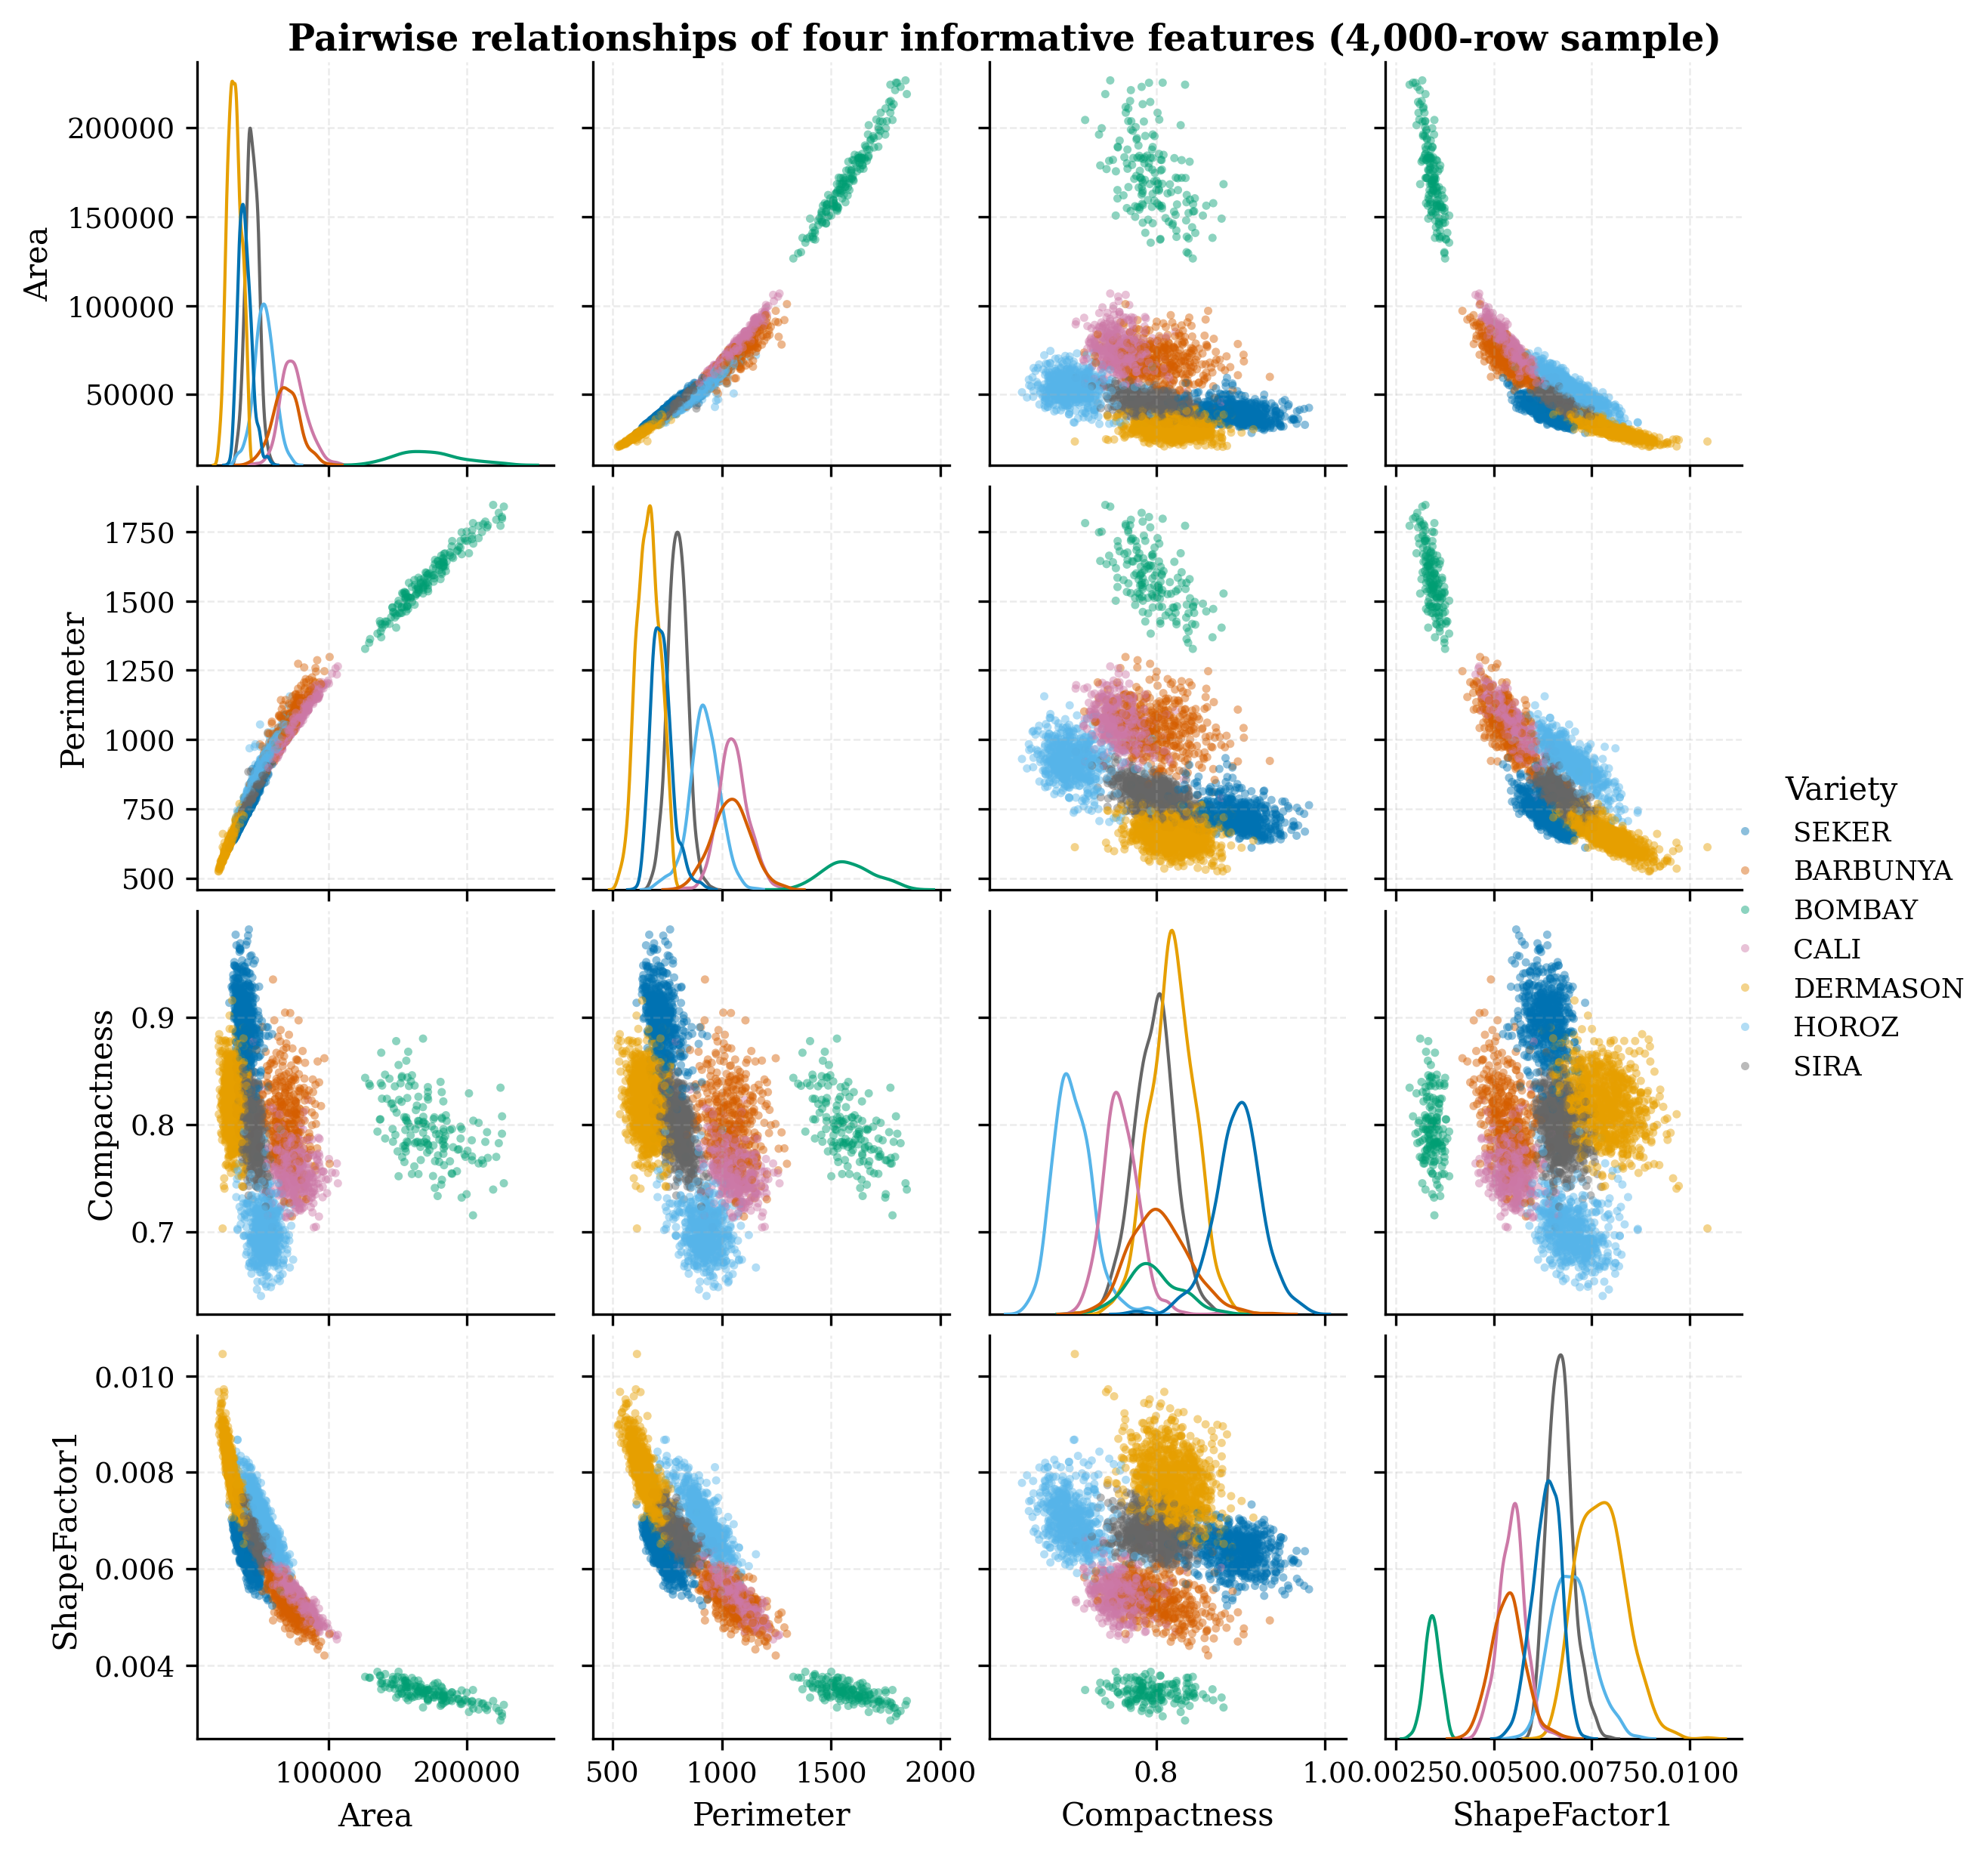
\includegraphics[width=0.62\textwidth]{fig_3_6_pairplot.png}
\caption{Pairwise relationships of four informative features on a 4,000-bean
sample. Two varieties separate cleanly; five overlap in a single cloud.}
\label{fig:pairplot}
\end{figure}

\begin{figure}[htbp]
\centering
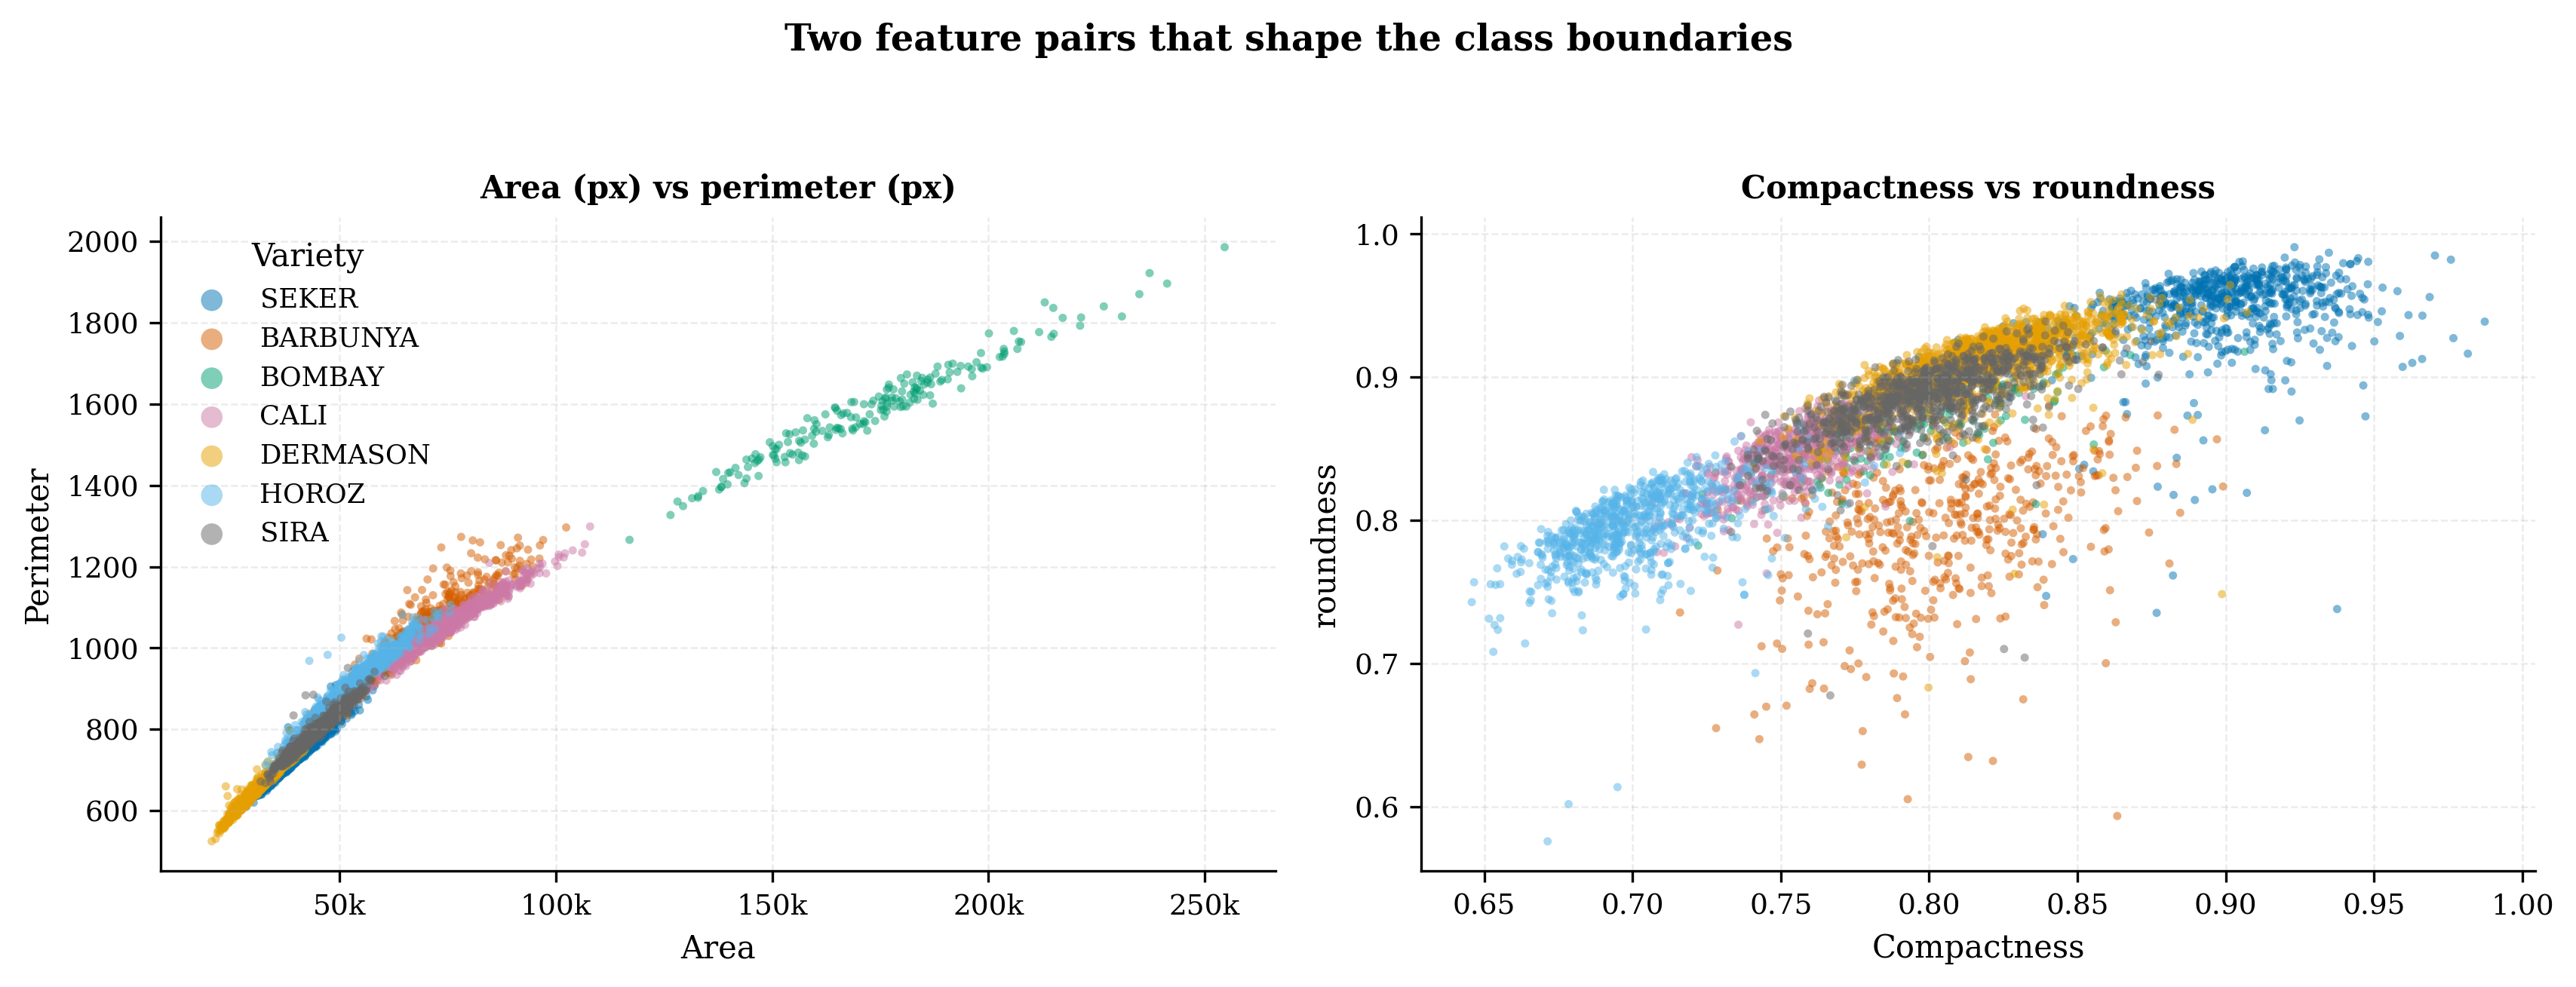
\includegraphics[width=0.92\textwidth]{fig_3_8_scatter_relationships.png}
\caption{Two feature pairs. Area and perimeter are almost collinear, so they
encode size twice; compactness and roundness separate the overlapping varieties.}
\label{fig:scatter}
\end{figure}

\subsection{Outliers}

Tukey's rule with a 1.5 IQR fence flags between 91 (\texttt{roundness}) and 843
(\texttt{Eccentricity}) observations per feature; Figure~\ref{fig:outliers} shows
the counts and the standardised spread. Almost all flagged points are large beans,
which belong to Bombay, rather than implausible measurements. No value falls
outside the physical range implied by the imaging setup, and there is no evidence
of a data-entry error: the size features are internally consistent
($\text{Area} \approx \pi E_d^2/4$ holds throughout).

Removing them would therefore delete the variety that is easiest to classify and
would bias the model against large beans. The outliers were retained. This is a
deliberate decision, not an oversight, and it is revisited as a limitation in
Section~7.2: a model trained without them would be less able to recognise an
unusually large Seker, but also less likely to mistake a Bombay for something
else.

\begin{figure}[htbp]
\centering
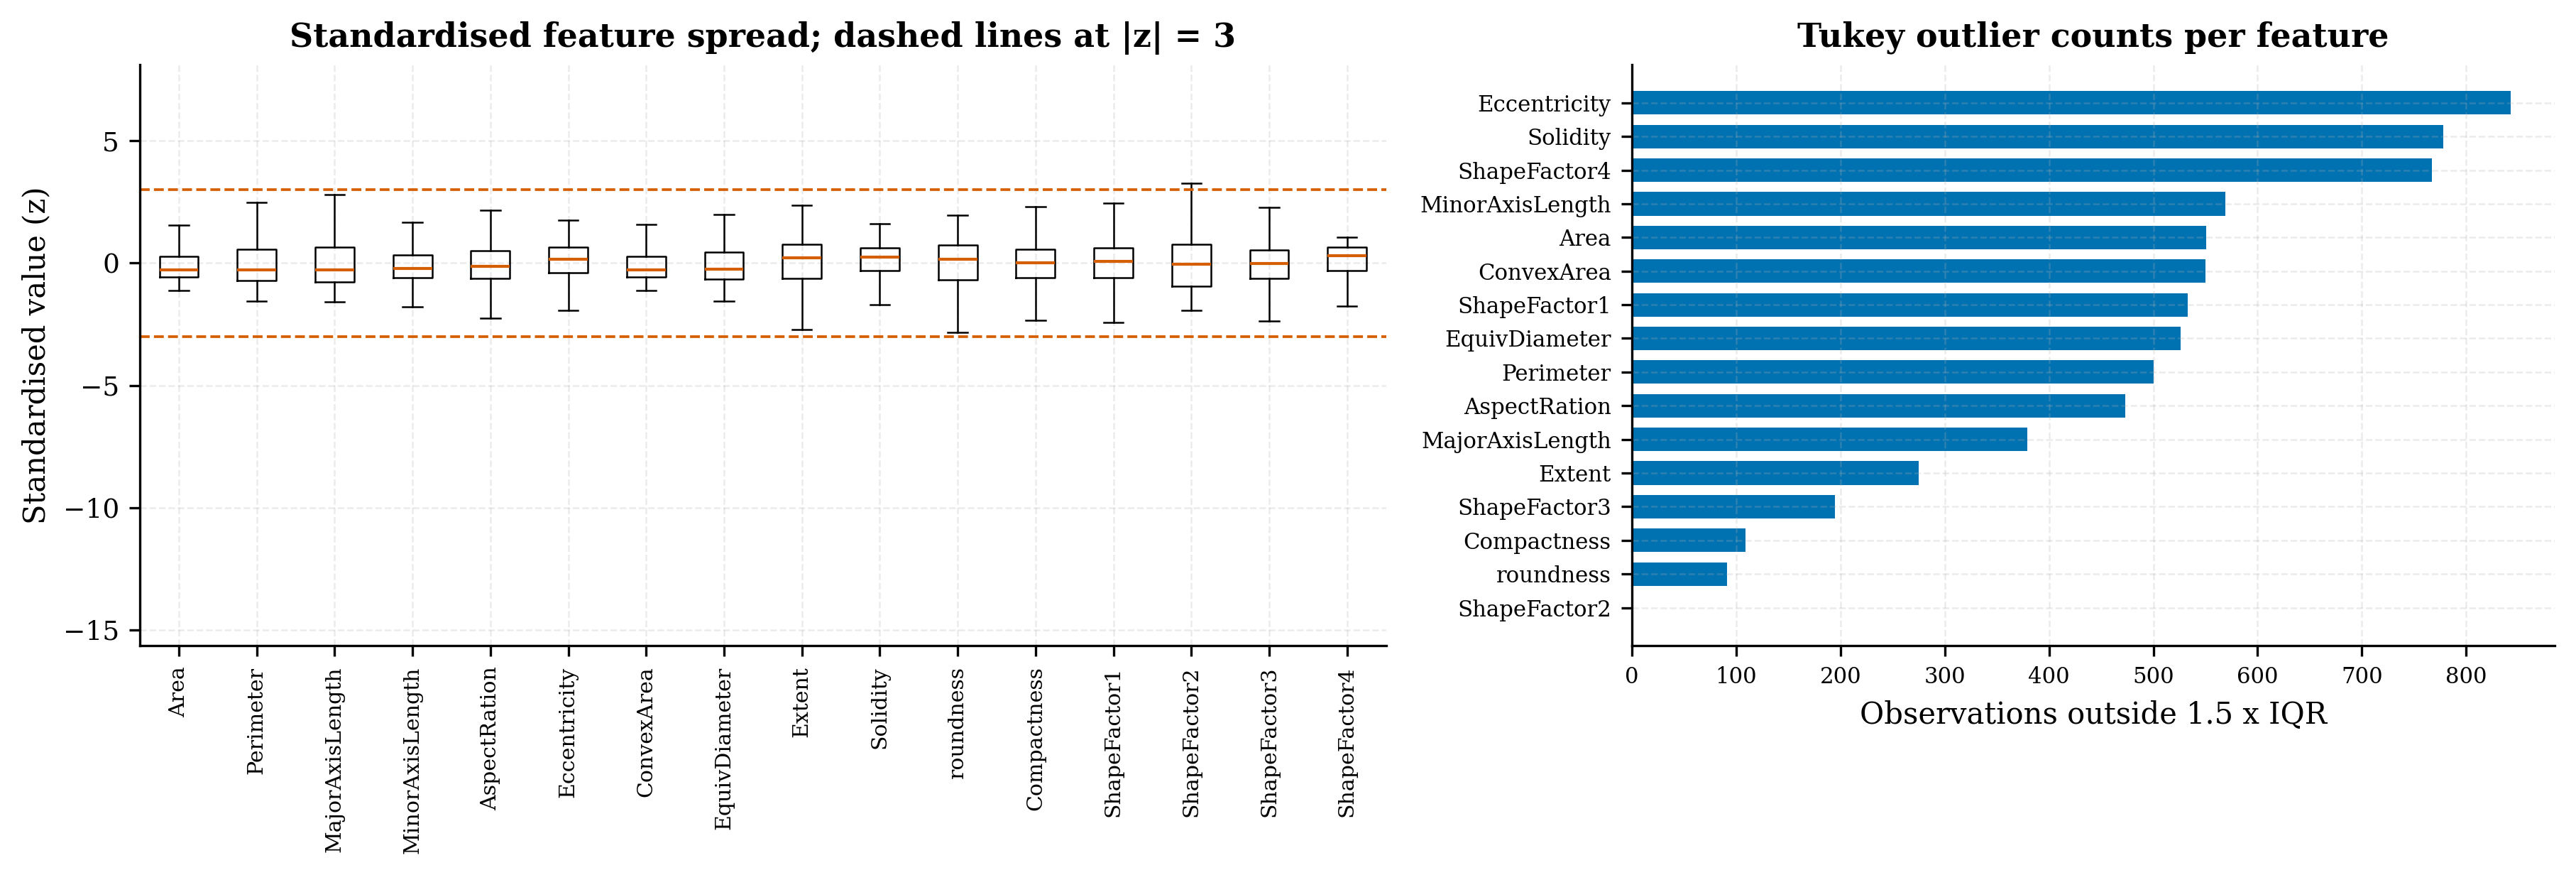
\includegraphics[width=0.92\textwidth]{fig_3_9_outlier_analysis.png}
\caption{Outlier analysis. Left: standardised spread with $\pm 3$ reference lines.
Right: Tukey outlier counts per feature. Flagged points are genuine large beans,
not measurement errors.}
\label{fig:outliers}
\end{figure}

\subsection{Discriminative power}

Figure~\ref{fig:anova} ranks the features by a one-way ANOVA $F$-statistic
computed across the seven classes. This is a descriptive statistic about the data,
not a model output, and it is used only to decide which features deserve a
dedicated plot. The size features lead, which is expected given Bombay, followed
by \texttt{ShapeFactor1} and \texttt{Compactness}. \texttt{Solidity} and
\texttt{ShapeFactor4} rank last, consistent with their narrow ranges.

\begin{figure}[htbp]
\centering
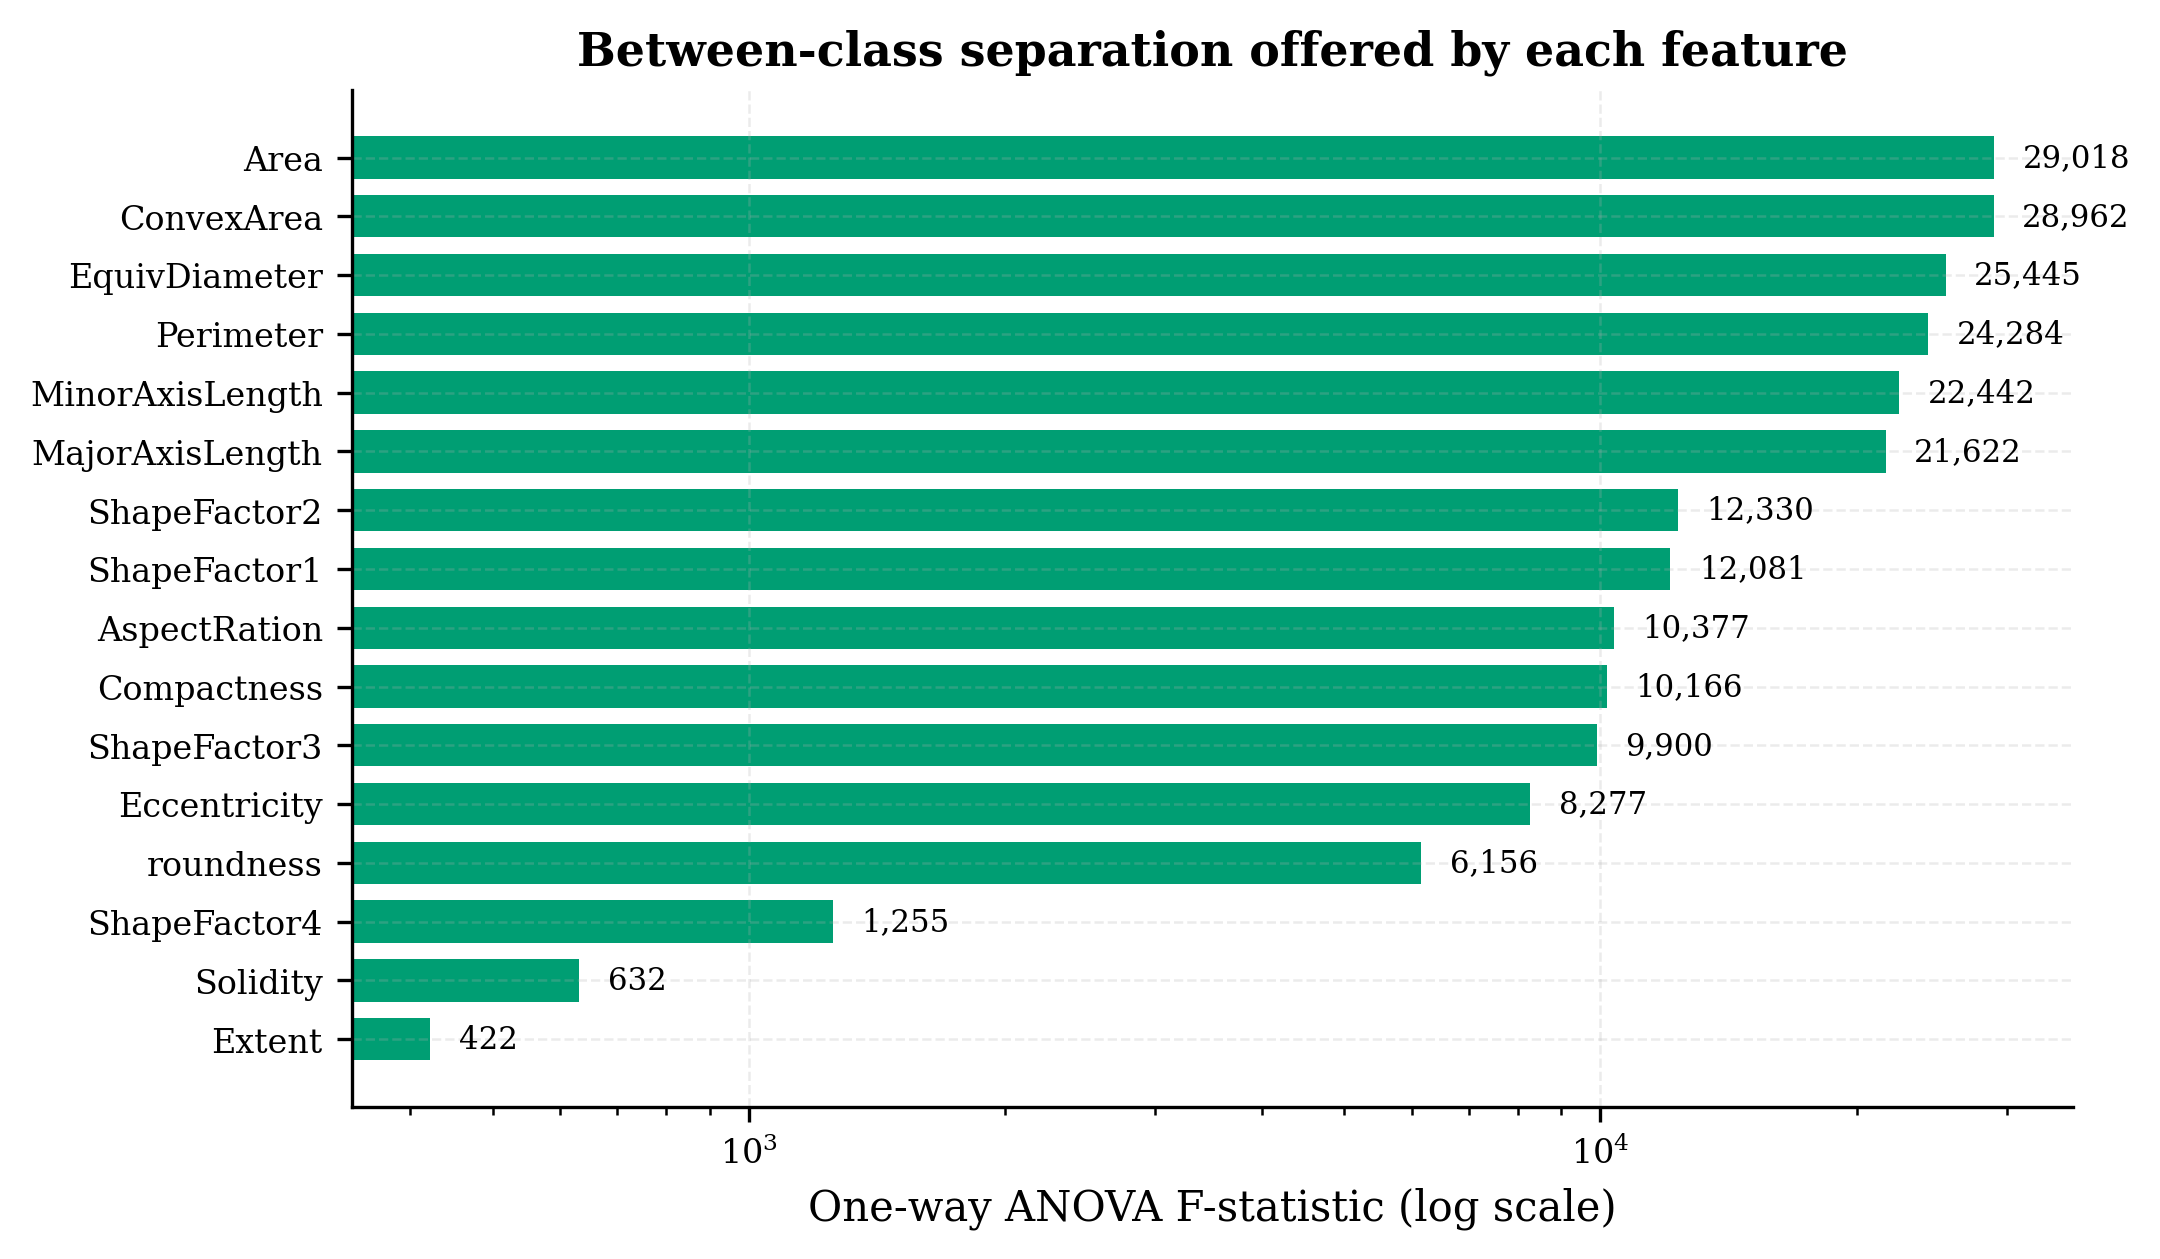
\includegraphics[width=0.66\textwidth]{fig_3_10_discriminative_power.png}
\caption{Between-class separation offered by each feature, measured by a one-way
ANOVA $F$-statistic on a logarithmic scale.}
\label{fig:anova}
\end{figure}

\section{Observations from EDA}

Six observations carried into the modelling stage.

\begin{enumerate}[label=(\roman*)]
  \item The classes are imbalanced by \ImbalanceRatio, so macro F1 is the
        selection metric and accuracy is reported only as a secondary figure.
  \item Bombay and Dermason are separated by size alone; the discrimination
        problem is concentrated in the five remaining varieties.
  \item Feature magnitudes span four orders of magnitude, so distance- and
        margin-based learners require standardisation, while tree ensembles do
        not.
  \item Twenty-one feature pairs exceed $|r| = 0.90$ because the shape factors are
        algebraic functions of the size features. Redundancy is a property of the
        data, and its effect on generalisation is measured, not assumed.
  \item The heavy right tails are genuine large beans. No observation was
        removed, and no transformation was applied, because the tree ensembles
        are insensitive to monotone transformations and the scaled models
        standardise anyway.
  \item The overlap between Cali, Barbunya, Sira and Horoz predicts a specific
        error pattern. Chapter~6 checks whether that prediction holds.
\end{enumerate}
